\chapter{苹果基因与蔷薇科植物基因可视化对比验证}
	\chaptermark{苹果基因与蔷薇科植物基因可视化对比验证}
	\section{拟南芥基因可视化}
		\subsection{拟南芥基因配置文件编写}
		拟南芥配置文编写分为两个部分,GBrowse全局配置文件编写,拟南芥数据源配置文件编写。首先GBrowse全局配置文件中需添加拟南芥数据源配置文件的信息。
		\begin{lstlisting}[language=bash]
		[malus_genome]
		description  = Malus Domestica1.0 database
		path         = malus.conf
		\end{lstlisting}
		其次,编写拟南芥数据源配置文件。
		\begin{lstlisting}[language=bash]
		[arabidopsis:database]
		db_adaptor    = Bio::DB::SeqFeature::Store
		db_args       = -adaptor DBI::mysql
		-dsn    dbi:mysql:database=blastx_arab_chr5;host=localhost
		-user   root
		-pass   root
		\end{lstlisting}
		最后,通过配置基因组的特征属性使用户可以通过Web浏览器看到可视化结果。
		\begin{lstlisting}[language=bash]
		[arabidopsis]
		feature      = match
		database     = arabidopsis
		glyph        = transcript2 
		bgcolor      = aqua
		height       = 8
		label        = 1
		key          = Arabidopsis Protein Alignments
		\end{lstlisting}
		\subsection{拟南芥基因组可视化结果}
		对拟南芥基因组的第五条染色体可视化结果,如图5.1。
		\begin{figure}[!ht]
			\centering
			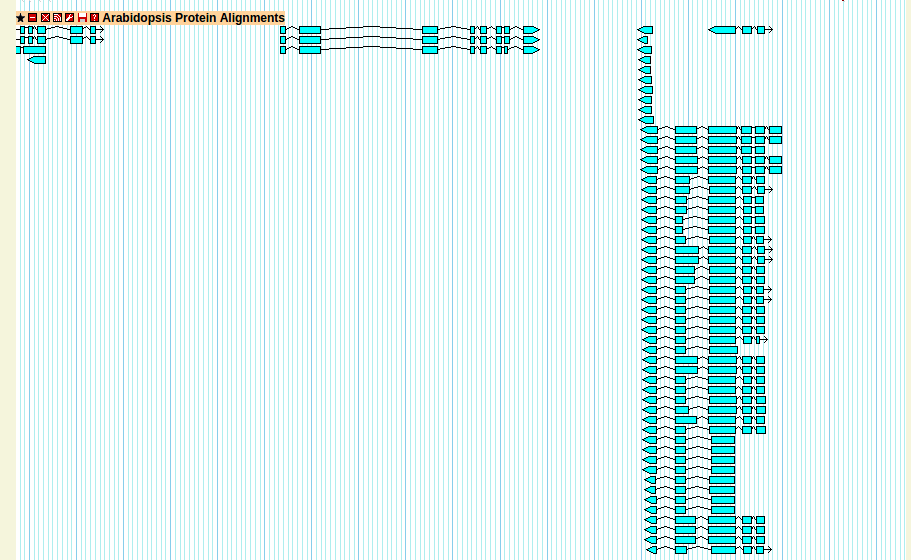
\includegraphics[width = .6\textwidth]{5-1.png}
			\caption{拟南芥基因可视化结果}
		\end{figure}
	\section{红桃基因可视化}
		\subsection{红桃基因配置文件编写}
		红桃配置文编写分为两个部分,GBrowse全局配置文件编写,红桃数据源配置文件编写。首先GBrowse全局配置文件中需添加红桃数据源配置文件的信息。
		\begin{lstlisting}[language=bash]
		[malus_genome]
		description  = Malus Domestica1.0 database
		path         = malus.conf
		\end{lstlisting}
		其次,编写红桃数据源配置文件。
		\begin{lstlisting}[language=bash]
		[peach:database]
		db_adaptor    = Bio::DB::SeqFeature::Store
		db_args       = -adaptor DBI::mysql
		-dsn    dbi:mysql:database=blastx_peach_chr5;host=localhost
		-user   root
		-pass   root
		\end{lstlisting}
		最后,通过配置基因组的特征属性使用户可以通过Web浏览器看到可视化结果。
		\begin{lstlisting}[language=bash]
		[peach]
		feature      = match
		database     = peach
		glyph        = transcript2 
		bgcolor      = limegreen
		height       = 8
		label        = 1
		key          = Peach Protein Alignments
		\end{lstlisting}
		\subsection{红桃基因可视化结果}
		对红桃基因组的第五条染色体可视化结果,如图5.2。
		\begin{figure}[!ht]
			\centering
			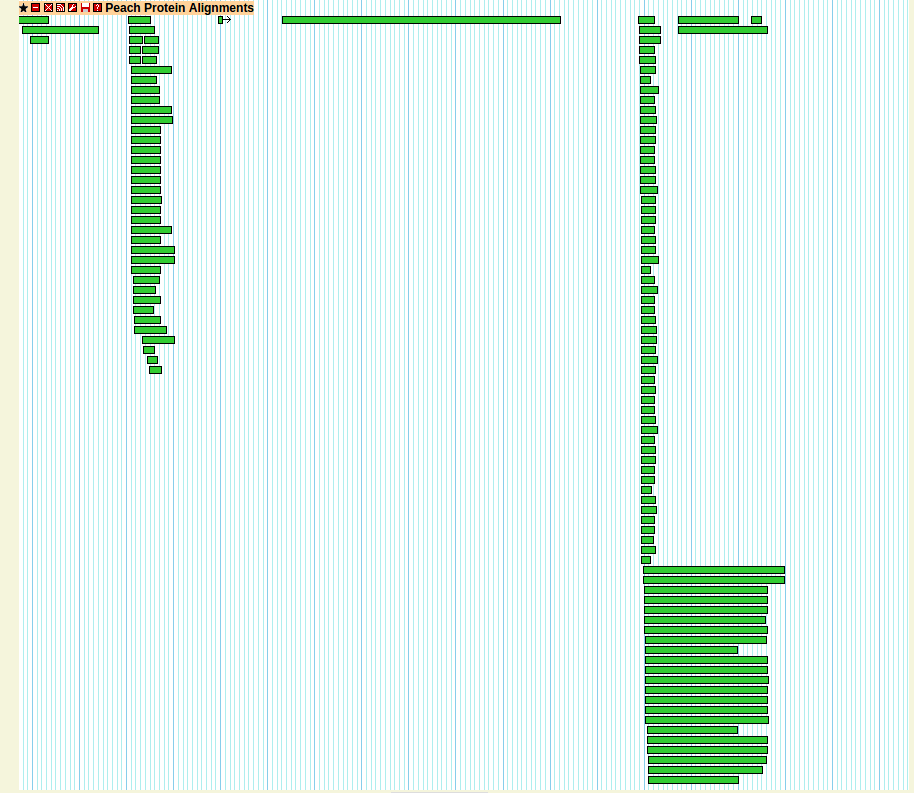
\includegraphics[width = .6\textwidth]{5-2.png}
			\caption{红桃基因可视化结果}
		\end{figure}
	\section{验证实验结果}
	在GBrowse中通过对苹果基因组的可视化可以使用户方便直观的查看到基因组的性状特征,通过对拟南芥及红桃基因组研究成熟基因组进行对比,可以是用户更加直观和方便的发现,苹果基因组相关功能的信息。
	
		